\section{Simulation}
For at teste den kontinuere controller's respons modelleres systemet ud fra state space repræsentationen og de fundne K-værdier til følgede blokdiagram uden brug af observer i første omgang. 

\begin{figure}[H]
	\centering
	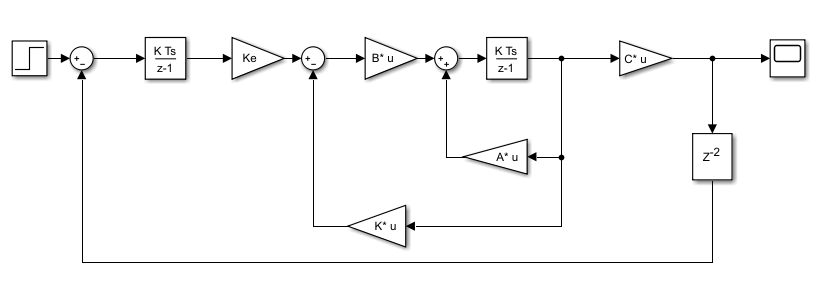
\includegraphics[width = 0.9\textwidth]{figur/Simulink_blokdiagram_1}
	\caption{Blok diagram for den kontinuere controller uden observer}
	\label{fig:Simulink_blokdiagram_1}
\end{figure}

State matricen hentes direkte fra modellen ligesom i Mathlab. Delay blokken med 2 unit delay skyldes at gerne vi simulere at gyroskopet på udgangen bruger 1 delay på at sample og og 1 delay på at integrere den samplede værdi.
Ved at sende et step med amplituden 30 ind som reference signal forventer vi derfor at kunne måle en værdi på 30 på outputtet efter cirka 1 sekund efter steppet. Dette kan ses i scopet 

\begin{figure}[H]
	\centering
	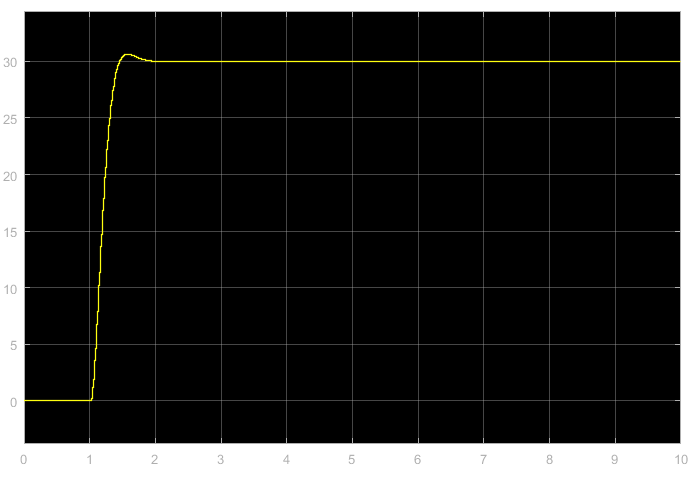
\includegraphics[width = 0.8\textwidth]{figur/Simulink_scope_1}
	\caption{Step respons for den kontinuere controller uden observer}
	\label{fig:Simulink_scope_1}
\end{figure}

Resultatet passer med forventningerne med settling time, overshoot og ingen steady state error. Men som nævnt tidligere kan man ikke hente disse states direkte ud fra systemet, så derfor tilføjes en observer til blokdiagrammet i \autoref{fig:Simulink_blokdiagram_1} så state matrixen kan hentes fra outputtet i stedet. Dette kan ses herunder.

\begin{figure}[H]
	\centering
	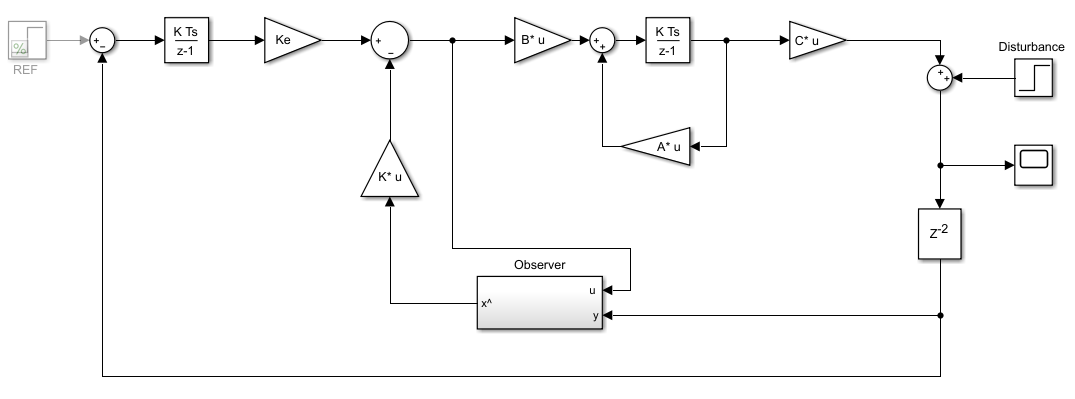
\includegraphics[width = 0.9\textwidth]{figur/Simulink_blokdiagram_2}
	\caption{Blok diagram for den kontinuere controller uden observer}
	\label{fig:Simulink_blokdiagram_2}
\end{figure}